\chapter{Laboratorio:  Programación de variadores de frecuencia y arrancadores suaves.}

\section{\obj}
\capacidad
\begin{itemize}
	{\small
    \item  Alambrar el circuito de control y potencia del variador.
    \item  Programar un variador de frecuencia segun los requerimientos. 
	\item Alambrar el arrancador suave para un motor trifásico.
	\item Alambrar un arranque pare reversible usando un arrancador suave de un motor trifásico.
	\item Programar el variador de frecuencia.
	\item Medir el tiempo de las rampas de aceleración y desaceleración, y vincular con los parámetros programados.
 }
\end{itemize} 

 
\section{Equipos y materiales}
Para este laboratorio de necesitaran:
\begin{itemize}
	{\small \item 1 motor trifásico 1/2 hp de 3 puntas.
	\item 1 variador de frecuencia: \href{https://search.abb.com/library/Download.aspx?DocumentID=3AUA0000066143&LanguageCode=en&DocumentPartId=1&Action=Launch}{ABB ACS355} o \href{https://vfds.com/content/manuals/delta/delta-vfd-el-manual.pdf}{VFD-EL}
	\item 1 arrancador suave SIEMENS RW3013.
	\item 2 contactores.
	\item 1 botón pulsar cerrado.
	\item 2 botones pulsadores abiertos.
	\item 3 interruptores N.O.
	\item 1 amperimetro de gancho con medición INRUSH.
	\item 1 analizador de señales trifásico FLUKE 143B.
}
\end{itemize}

\section{Marco de referencia}


Los arrancadores suaves son sistemas electrónicos de control de motores que permiten arrancar y parar motores asíncronos de inducción. Los arrancadores suaves disponen de dos tiristores conectados en antiparalelo en dos de las tres fases como se muestra en la Figura \ref{fig:controlfase}. La corriente en la tercera fase no controlada, es una suma de las corrientes de las dos fases controladas. El arrancador suave realiza un recorte del angulo $\alpha$ en cada fase, por lo tanto, la tensión del motor aumenta desde un voltaje inicial hasta la tensión a plena carga en un tiempo definido por el usuario. La tensión de inicio y el tiempo de la rampa se relacionan según la Figura \ref{fig:rampasarrancador} y estos parámetros son ajustados mediante los dos potenciometros de la Figura \ref{fig:3rw3013-1bb14gic03xx31074p} .

La intensidad del motor tiene un comportamiento proporcional a la tensión aplicada al motor. De este modo, la corriente de arranque se reduce en el mismo factor que la tensión aplicada al motor. La Figura \ref{fig:corrientemotor} muestra la reducción en la corrientes. Por otra parte, el torque tiene un comportamiento cuadrático respecto a la tensión aplicada al motor. La Figura \ref{fig:torquemotor} muestra como el par de arranque se reduce de forma cuadrática con la tensión aplicada al motor. En ambos casos se aprecia las curvas de corrientes y torque con rampas de tiempo cortas o prolongadas.

\begin{figure}
	\centering
	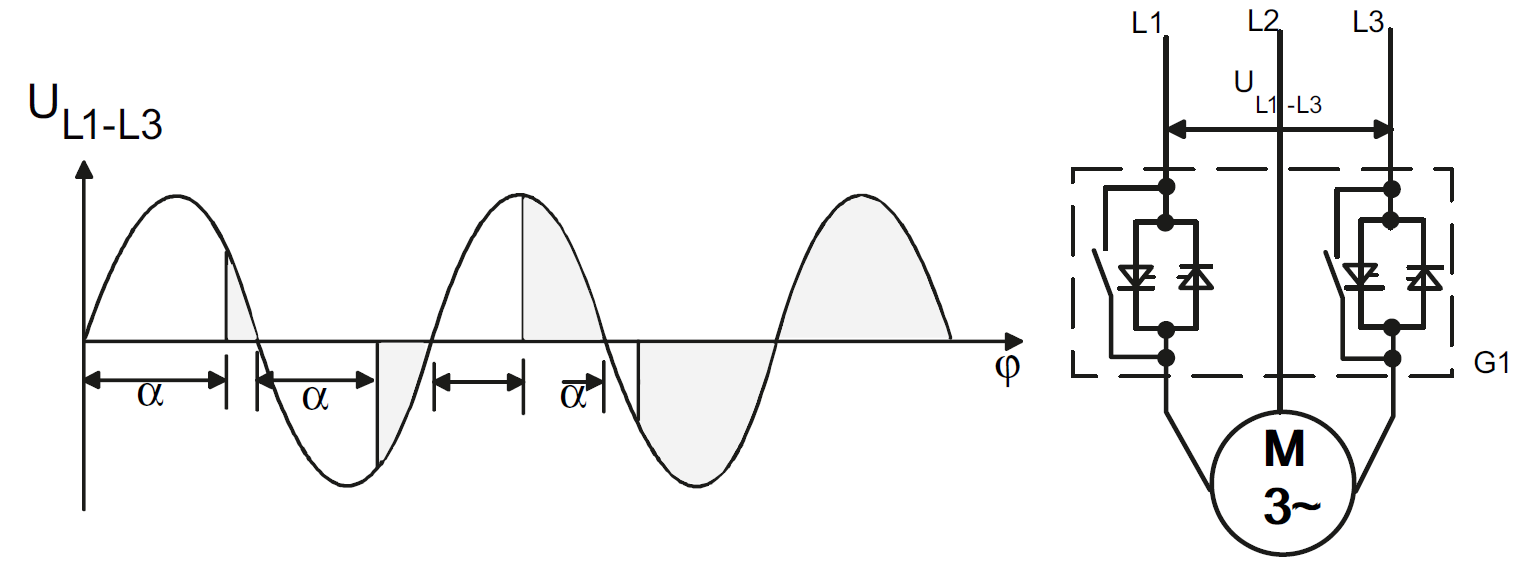
\includegraphics[width=0.75\linewidth]{fig/ControlFase}
	\caption{Control por recorte de fase y esquema de un arrancador suave con control bifásico. \cite{SIEMENS}}
	\label{fig:controlfase}
\end{figure}



\begin{figure}
	\centering
	\begin{subfigure}[b]{0.69\textwidth}
		\centering
		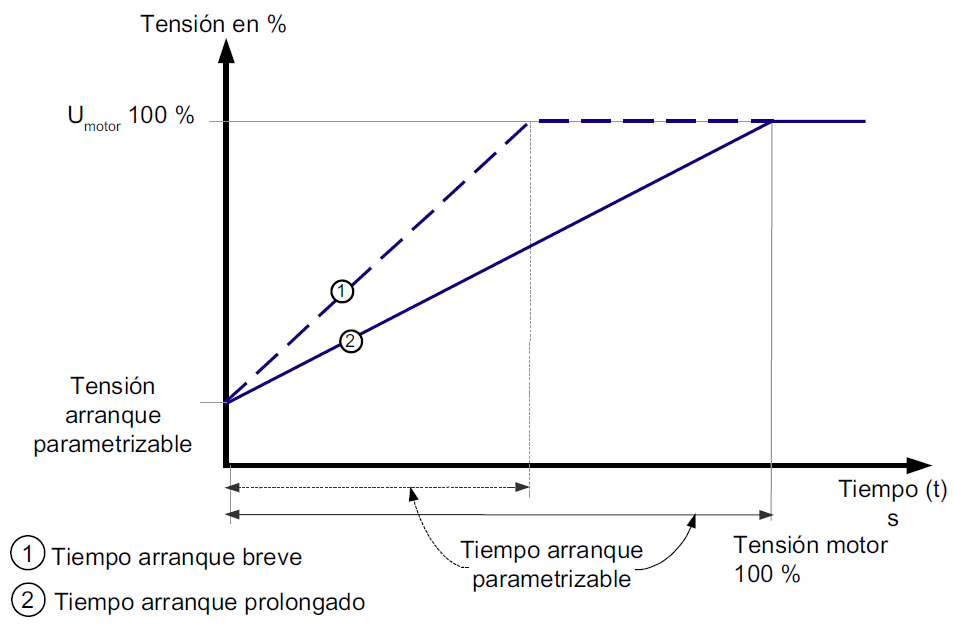
\includegraphics[width=\textwidth]{fig/RampasArrancador}
		\caption{Principio de funcionamiento}
		\label{fig:rampasarrancador}
	\end{subfigure}
	\hfill
	\begin{subfigure}[b]{0.3\textwidth}
		\centering
		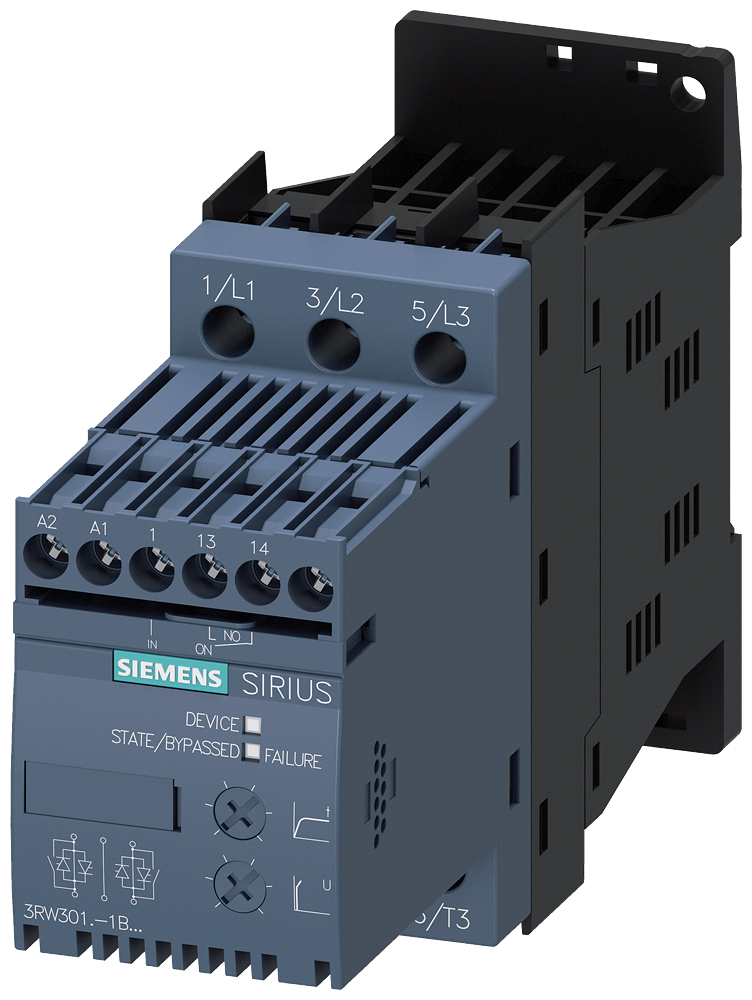
\includegraphics[width=\textwidth]{fig/3RW3013-1BB14_G_IC03_XX_31074P}
		\caption{Imagen del arrancador}
		\label{fig:3rw3013-1bb14gic03xx31074p}
		
	\end{subfigure}
	\caption{Arrancador suave SIEMENS 3RW3013.\cite{SIEMENS}}
\end{figure}


\begin{figure}
	\centering
	\begin{subfigure}[b]{0.49\textwidth}
		\centering
		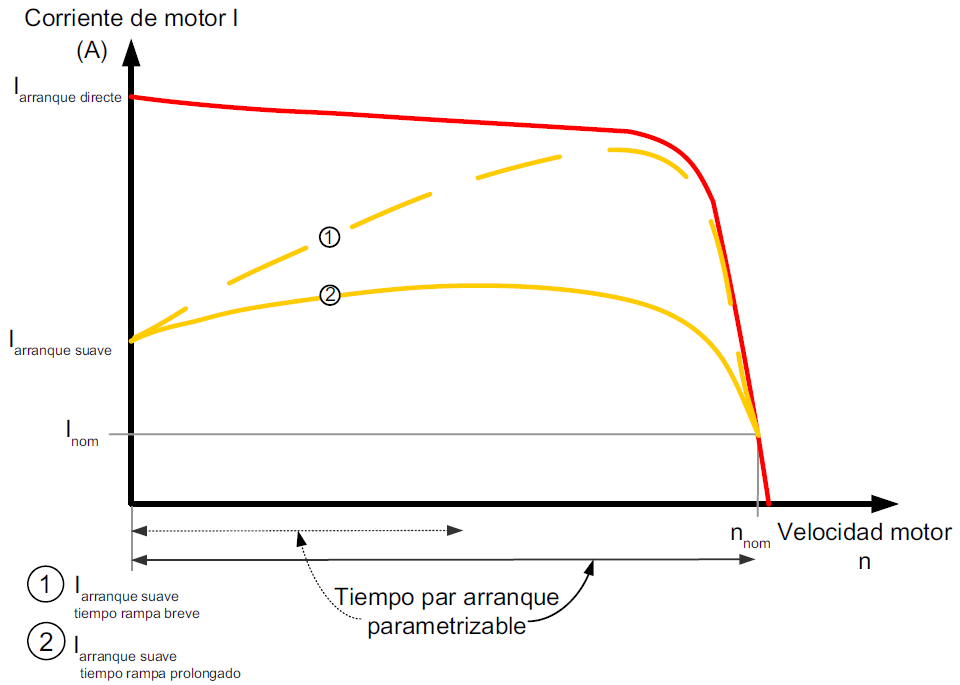
\includegraphics[width=\textwidth]{fig/CorrienteMotor}
		\caption{Corrientes del motor}
		\label{fig:corrientemotor}
	\end{subfigure}
	\hfill
	\begin{subfigure}[b]{0.49\textwidth}
		\centering
		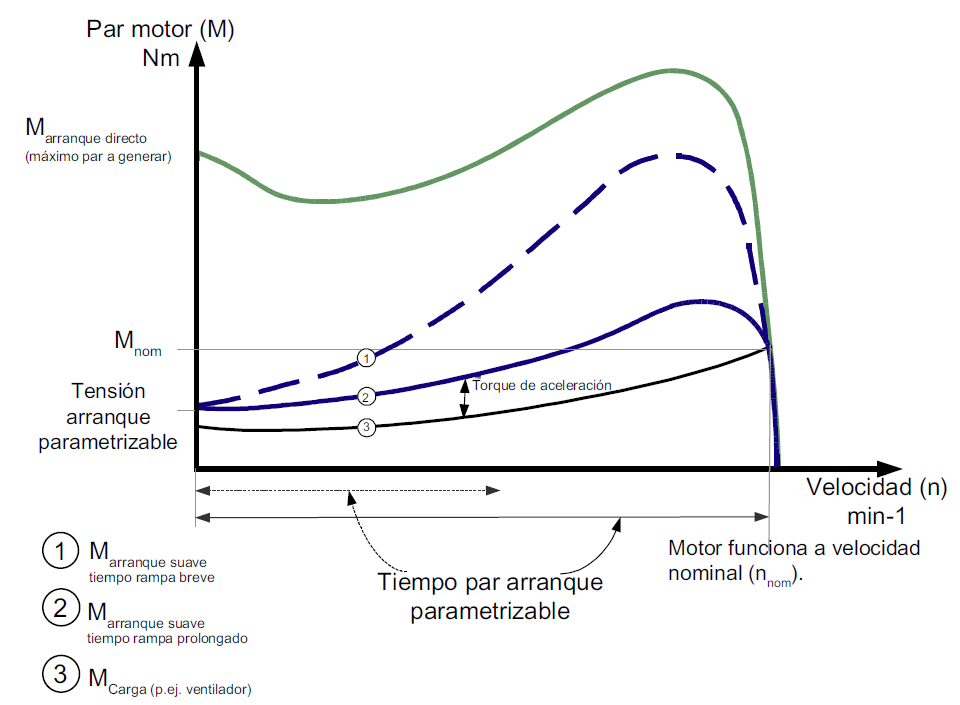
\includegraphics[width=\textwidth]{fig/TorqueMotor}
		\caption{Torque del motor}
		\label{fig:torquemotor}
		
	\end{subfigure}
	\caption{Curvas de corrientes y torques versus velocidad.\cite{SIEMENS}}
\end{figure}



\subsection{Variadores de Frecuencia}

Un variador de frecuencia (VDF) es un dispositivo que se utiliza para controlar la velocidad y el par de un motor eléctrico alterando la frecuencia y el voltaje suministrado al mismo. El VDF es capaz de convertir la corriente alterna (CA) de entrada, en una señal de pulsos alternos con frecuencia y voltaje adecuados para el motor. Esta señal de salida se llamada modulación por ancho de pulso (PWM). La Figura \ref{fig:pwm} muestra señales PWM que equivalentes a señales sinosoidales de: a) 60 Hz y 120V, b)30Hz y 60V, c) 20Hz y 40V.

\begin{figure}
	\centering
	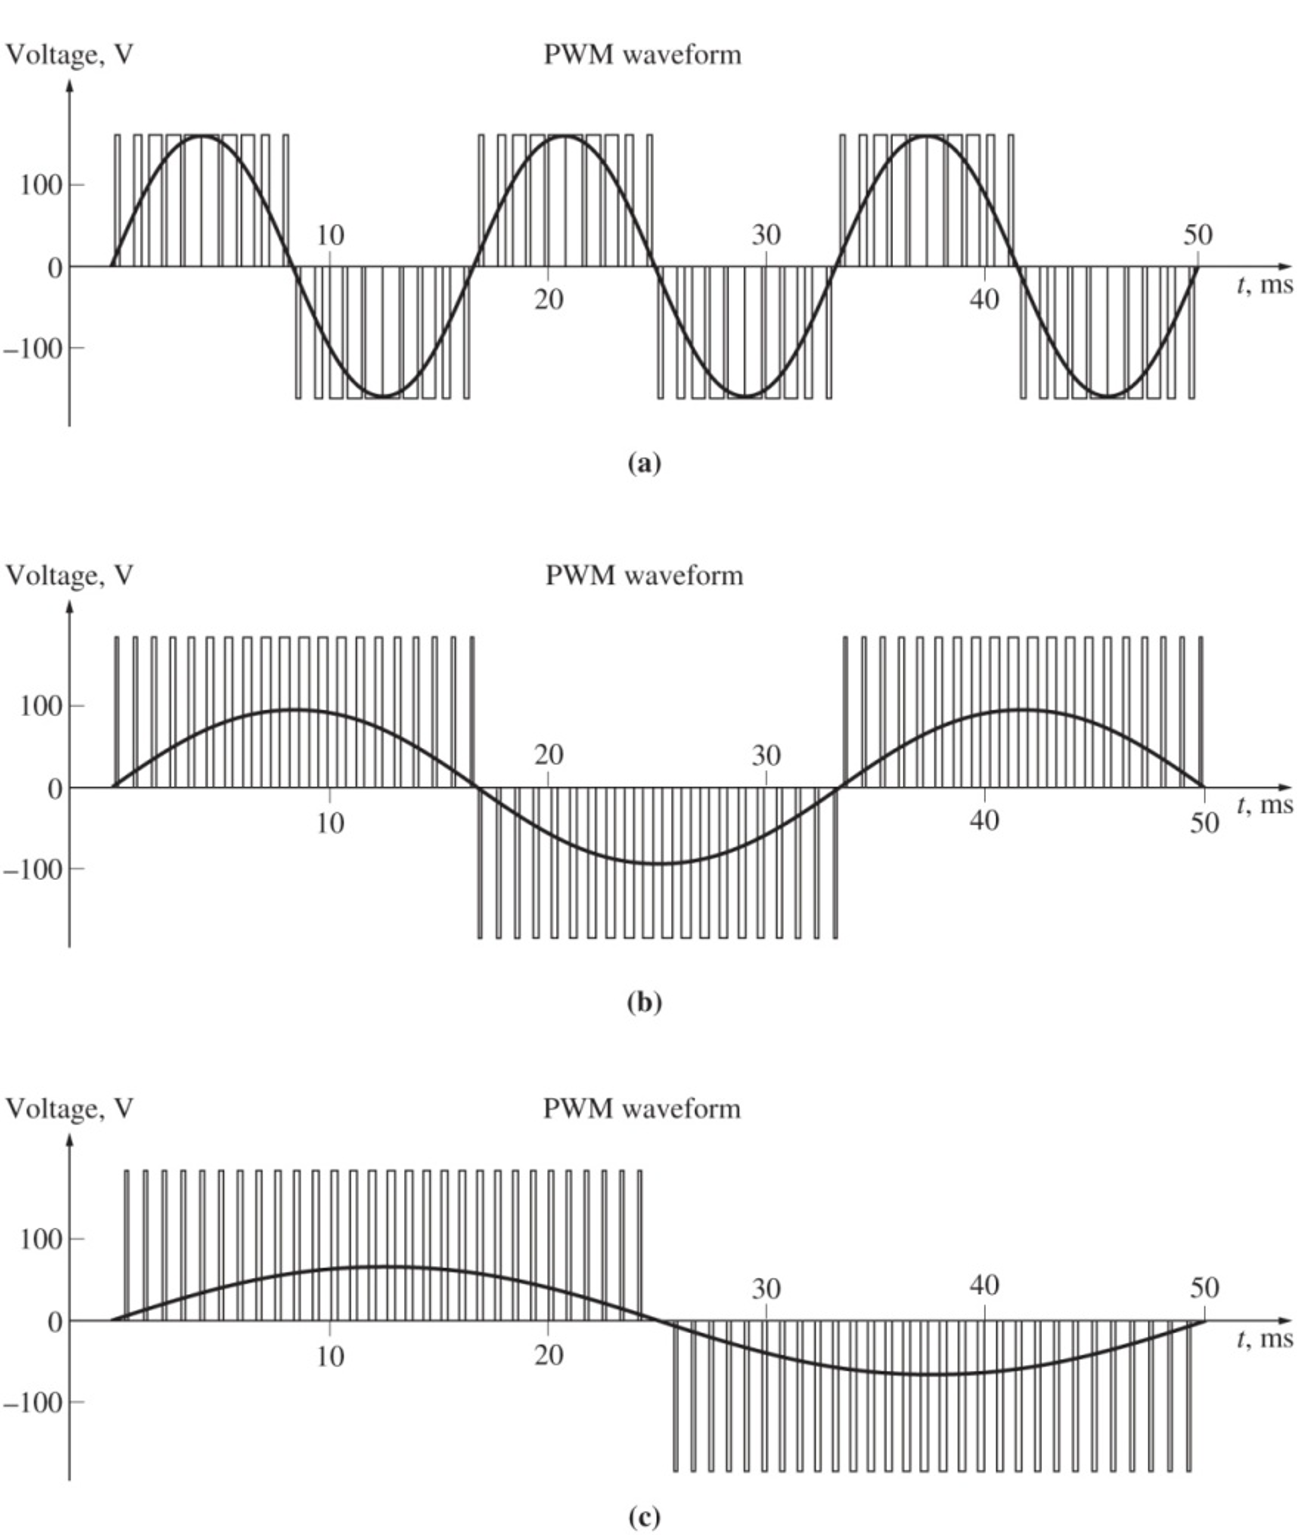
\includegraphics[width=0.8\linewidth]{fig/pwm2}
	\caption{Señales PWM equivalentes a señales sinosoidales de distintas amplitud y frecuencia \cite{Chapman12}.}
	\label{fig:pwm}
\end{figure}


El variador de frecuencia permite variar la velocidad del motor eléctrico en función de las necesidades de la aplicación, lo que puede resultar en un ahorro de energía y un mayor control de la velocidad. Además, el variador de frecuencia también puede proporcionar protección al motor, ya que puede detectar y proteger contra situaciones de sobrecarga, cortocircuito y fallos de fase, entre otros problemas.

Un VDF puede operar bajo dos principios: el control escalar y control vectorial \cite{Posadas05}. El control escalar, también conocido como control $V/f$ (voltaje/frecuencia), es el método de control más simple y comúnmente utilizado en los variadores de frecuencia. En este método, se ajusta la frecuencia y el voltaje de salida del variador en función de la carga del motor para mantener una relación de flujo magnético constante equivalente a la relación $V/f$. El control escalar es más adecuado para aplicaciones que requieren un control de velocidad básico, como ventiladores y bombas. 

Por otra parte, el control vectorial, conocido como control de campo orientado, es una técnica de control avanzada que permite un mayor grado de precisión en el control del motor. En este método, se utiliza un modelo matemático del motor para controlar tanto la velocidad como el par del motor de manera independiente. Esto se logra mediante el control de la corriente y el voltaje en el estator del motor, lo que permite un control preciso de la orientación del campo magnético del motor. El control vectorial es más adecuado para aplicaciones que requieren un control de velocidad preciso y una alta dinámica, como en máquinas herramienta y robots industriales.

\subsection{Partes del variador}

La Figura \ref{fig:ab160} muestra las principales partes del VDF y se detallan a continuación:
\begin{enumerate}
	\item Rectificador: Es la parte que convierte la energía eléctrica de entrada en una señal de corriente directa (CD) que se utiliza como entrada para el inversor.
	
	\item Inversor: Es la parte que convierte la señal de corriente directa (CD) en una señal PWM con la frecuencia y el voltaje adecuados para el motor.
	
	\item Microprocesador: Es el cerebro del variador y controla todas las funciones y operaciones del mismo. El microprocesador recibe las señales de entrada y, en función de los parámetros de programación establecidos, envía las señales adecuadas al rectificador e inversor para controlar la velocidad y el par del motor.
	Adicionalmente el controlador se encarga de monitorear el variador, incluyendo la protección del motor contra sobrecargas, cortocircuitos, fallos de fase, etc.
	
	\item Interfaz de usuario: Es la parte que permite a los usuarios interactuar con el variador, configurar los parámetros de programación y monitorear su operación.
	
	\item Circuitos de medición: son los circuitos encargados de medir las variables eléctricas del variador y el motor, incluyendo la protección del motor contra sobrecargas, cortocircuitos, fallos de fase, etc.
	
\end{enumerate}

\begin{figure}
	\centering
	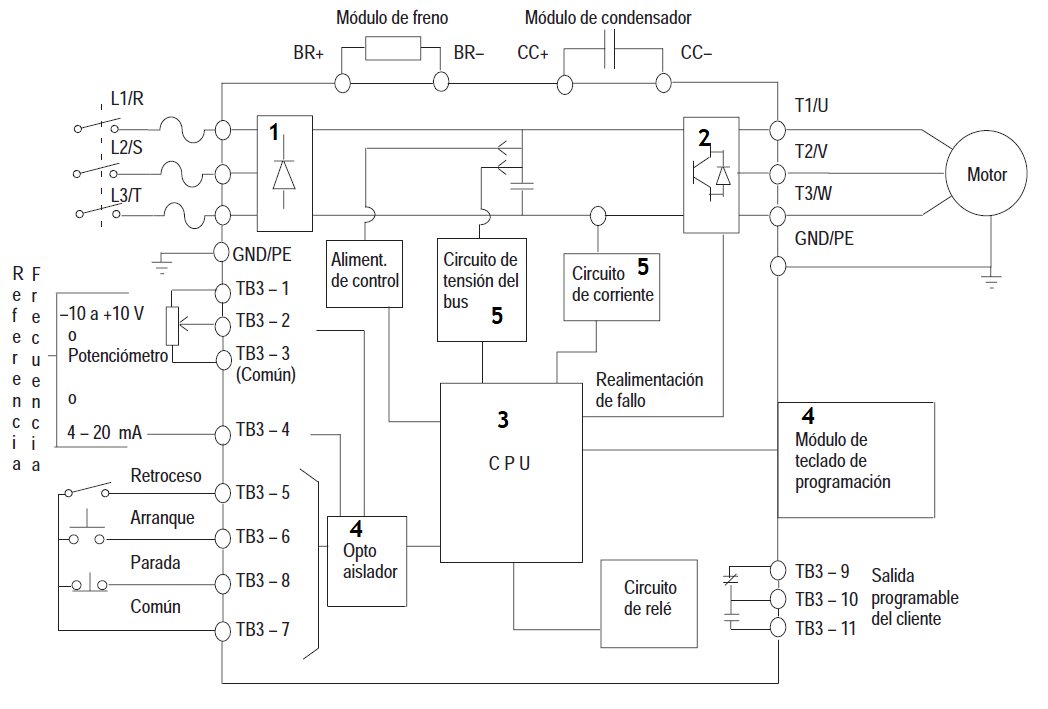
\includegraphics[width=0.9\linewidth]{fig/AB160}
	\caption{Esquema del Variador de Frecuencia AB160.\cite{AB160} }
	\label{fig:ab160}
\end{figure}

\subsection{Parámetros de programación}

 Los parámetros para configurar un VDF puede oscilar desde unos pocos parámetros básicos hasta cientos. Sin embargo los obligatorios son definidos por la red eléctrica, los datos de placa del motor y la aplicación. Entre ellos destaca: Tensión base o tensión nominal del motor, Frecuencia nominal del motor, frecuencia mínima y máxima de operación del motor,  modos de parada del motor , modos de entrada (cableado de entrada), modos de salida (relés de alarmas), tiempo de aceleración y desaceleración del motor y frecuencias restablecidas activadas por señales digitales.
 
Para el calculo de los  tiempos de aceleración y desaceleración se requiere conocer el torque del motor ($T_m$), el torque de la carga ($T_r$), la inercia total del sistema mecánico $J$, la velocidad angular  de inicio ($\omega_i$),  la velocidad angular final ($\omega_f$) y el delta de tiempo ($\Delta t$) que es el tiempo que se tarda entre ambas velocidades angulares. Por lo tanto el torque de aceleración ($T_A$) debe ser siempre menor al $150\% T_m$ de lo contrario existirán problemas de sobrecarga.

\begin{equation}
T_A=J\dfrac{(\omega_f-\omega_i)}{\Delta t} + T_r
\end{equation}

Si se asume que un motor de inducción  puede entregar un torque máximo de 150\% de su torque, entonces  las rampas de aceleración se calculan como:

\begin{equation}
\Delta t=J\dfrac{(\omega_f-\omega_i)}{1.5 T_m-T_r}
\end{equation}
 
 El tiempo natural en que se frena la inercia esta dado por \eqref{Eq:Tmin}, si se requiere frenar el sistema de forma más acelerada, es necesario colocar en el VDF resistencias que disipan la potencia eléctrica entregada por el motor, el cual se encuentra operando como alternador.
 
 \begin{equation}
 \Delta t=J\dfrac{\omega_i}{T_r}
 \label{Eq:Tmin}
 \end{equation}
 
 Por otra parte, la frecuencia de operación del VDF se selecciona según las necesidades mecánicas de la carga; por ejemplo, el motor de un reductor de velocidad debe operar a 950 revoluciones por minuto (rpm). Para determinar la frecuencia  que se debe programar, se requiere conocer el deslizamiento del motor ($s$), sus polos ($p$), la frecuencia nominal ($f_n$), el tipo o comportamiento de la carga (torques constantes, torques variables).
 
 Cuando el torque de la carga es constante, Figura \ref{fig:torqueconstante}, las velocidades de deslizamiento son contantes no importa la frecuencia en que opera el motor. Esto implica que el deslizamiento en el nuevo punto de operación($s_2$) está dado por, $s_2=s\cdot f_n/f_2$. Sabiendo que la velocidad mecánica está dada por:
 
 \begin{equation}
 	\eta_{mec}=\dfrac{120f_n}{p}(1-s)
\end{equation}
 entonces, la nueva frecuencia  ($f_2$) a programar el en VDF en función de la  velocidad mecánica deseada ($\eta_{mec2}$) se determina de la siguiente  forma,
 \begin{equation}
 f_2=\dfrac{p\left(\eta_{mec2}+ \dfrac{120sf_n}{p}\right) }{120}.
 \end{equation} 
 
 Las bombas centrifugas o abanicos  son ejemplos de par resistente variable, tal y como se aprecia en la figura \ref{fig:torquevariable}. En estos casos la velocidad de deslizamiento varia según la carga, pero una aproximación con error menor al 1\% asume que los deslizamientos son constantes, por tanto  $s_2=s$.
 
 
 \begin{figure}
 	\centering
 	\begin{subfigure}[b]{0.49\textwidth}
 		\centering
 		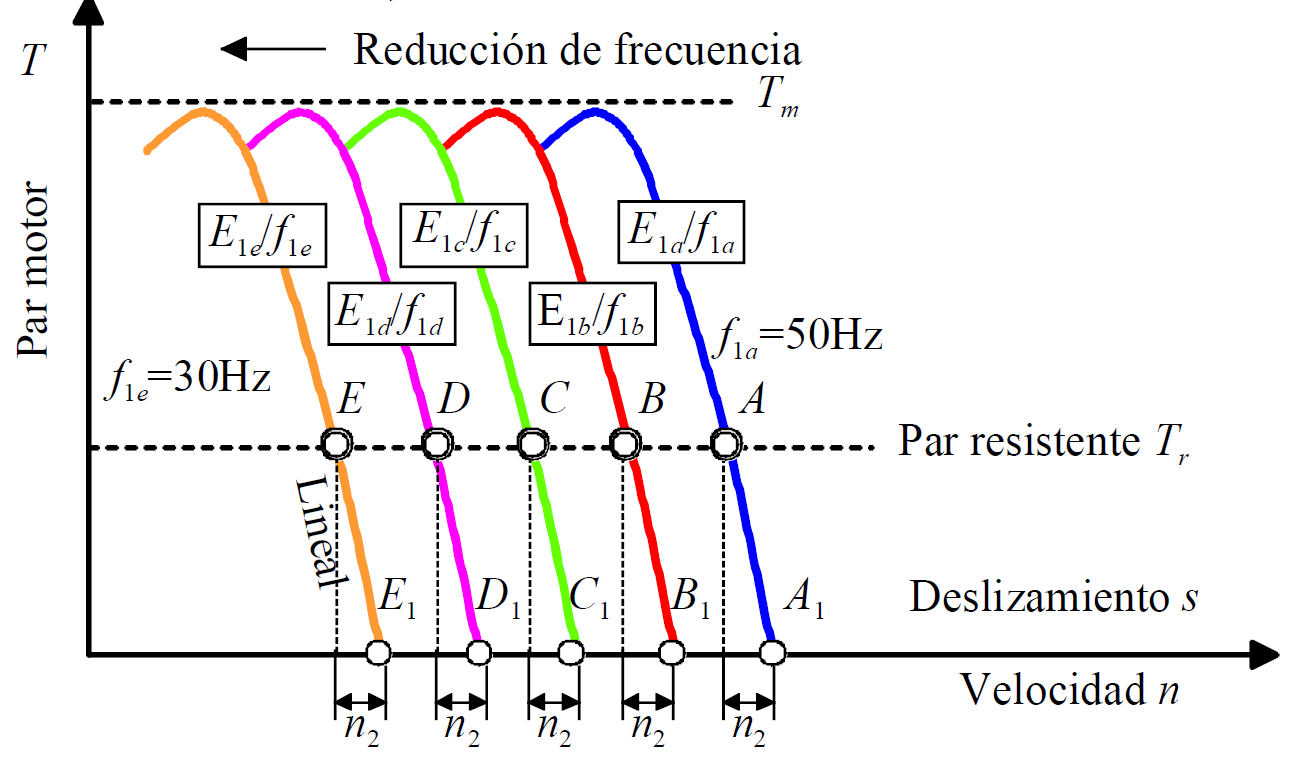
\includegraphics[width=\textwidth]{fig/TorqueConstante}
 		\caption{Torque carga constante}
 		\label{fig:torqueconstante}
 	\end{subfigure}
 	\hfill
 	\begin{subfigure}[b]{0.49\textwidth}
 		\centering
 		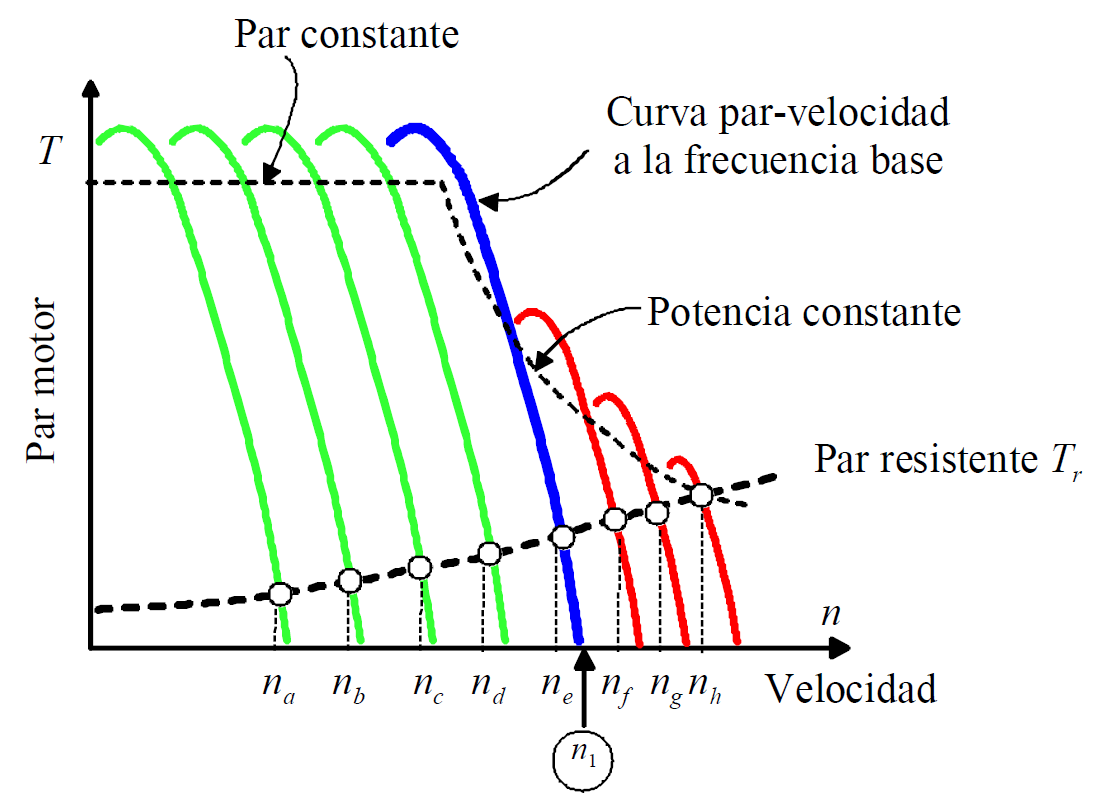
\includegraphics[width=\textwidth]{fig/TorqueVariable}
 		\caption{Torque de carga variable}
 		\label{fig:torquevariable}
 	\end{subfigure}
 	\caption{Curvas de torque inducido del motor y par de la carga. \cite{Mora08}}
 \end{figure}
 
 
 
\section{Metodología}

Este laboratorio tiene una duración de 4 lecciones, repartidas en dos semanas. Los estudiantes deben mostrar durante las clases programadas las tres actividades propuestas. Deben recabar fotografías y resultados de los equipos de medición para elaborar las evidencias. Las evidencias se subirán al TecDigital la semana siguiente finalizadas las actividades.

\section{Práctica en Clase}

\subsection{Actividad 1}

Suponga que el arrancador suave es para un motor de una cinta transportadora que puede operar en ambos sentidos. Según el manual del \href{https://support.industry.siemens.com/dl/files/095/38752095/att_1310813/v1/Manual_softstarter_3RW30_3RW40_es-MX.pdf}{SIRIUS 3RW30} \cite{SIEMENS}, sección 13.1.2, seleccione el voltaje de inicio y la rampa de tiempo recomendada.
Implemente un circuito de control y potencia para que el motor arranque en dos sentidos, para esto puede usar como referencia la sección 16 de ejemplos. 
 
\subsubsection{Conteste las preguntas}

¿Puede mostrar el circuito de control del sistema?
Usando un analizador Fluke 143B  mida la corriente de arranque del motor.
¿Como son las señales de corriente y voltaje a la entrada del motor con/sin arrancador suave?
¿Cuanto tiempo tardó en aparecer el voltaje de línea en las terminales?¿Coincide con la rampa de tiempo pre-establecida?

\subsection{Actividad 2}
 

Utilizando el manual del variador, encuentre el código que re-inicial el VDF a sus valores de fábrica.
Luego ingrese los parámetros descritos en la sección 3.3 asociados al voltaje, corriente nominal y frecuencia base del motor.
Posteriormente seleccione un modo de entrada que permita operar el motor en ambos sentidos mediante cableado externo.
Programe rampas de aceleración entre las frecuencias mínimas y máximas de 20 segundos y de desaceleración de 30.
Programe siete frecuencias en el VDF, asumiendo torque constante en vacío,de tal forma que en el eje del motor se midan las velocidades de la Tabla \ref{Tab:velocidades}.

\begin{table}[H]
	\centering  
	\caption{Velocidades solicitadas}
	\label{Tab:velocidades}
	\begin{tabular}{|c|c|}
		\hline 
		Velocidad	&	Rev/min	\\	\hline 
		
		0	&	900	  	   	 \\ 
		1	&	1050	  	   	 \\ 
		2	&	1200	  	   	 \\ 
		3	&	1350	  	   	 \\ 
		4	&	1500	  	   	 \\ 
		5	&	1650	    	 \\ 
		6	&	1800        	 \\ 
		7	&	1950     	   	 \\ 
		\hline 
	\end{tabular} 
\end{table}
 

 
\subsubsection{Conteste las preguntas:}

Realice la gráfica de voltaje en función de la frecuencia ($V=\mathfrak{F}(f)$), ¿Es como se esperaba?
Realice una tabla con las mediciones de las velocidades medidas, ¿Cuál fue el porcentaje de error relativo de cada medición?
Si se programa el variador con frecuencias calculadas con torque variable, los errores mejoran o empeoran? ¿Por qué?
¿Son las gráficas PWM a la salida del variador son como se esperan? ¿Puede mostrar un gráfico? Si se desconecta una fase de entrada en VDF, ¿que sucedió con el VDF? Mida las rampas de aceleración y desaceleración, cumple lo programado? Cuanto tarda de pasar de la velocidad 3 a la 5 y viceversa, tienen estos tiempos sentido? Que pasaría si se programan rampas de 1 segundo de aceleración y des-aceleración?
 

%\section{Informe de evidencias para el TECDIGITAL}
%
% Para cada actividad copie los resultados que se imprimieron en el puerto serial. Adicionalmente, para las actividades 2 y 3 muestre las fotografías de los circuitos.
% 
% El informe que se sube al TEC DIGITAL debe ser un archivo PDF, con las siguiente partes:
% 
% \begin{enumerate}
% 	\item Identificación del laboratorio, Autores, fecha.
% 	\item Resumen
% 	\item Objetivos
% 	\item Descripción de la actividad x.
% 	\item Evidencia fotográfica de los circuitos. 
% 	\item Evidencia de los resultados obtenidos (gráficas, tablas, imágenes, etc ).
% 	\item Análisis de las preguntas planteadas en la actividad.
% 	\item Referencias.
% \end{enumerate}
% 
% Si el laboratorio posee x actividades los pasos 4,5,6 y 7 se repiten x veces. 



